\documentclass[12pt,a4paper]{report}
\usepackage[italian, english]{babel}
\usepackage{newlfont}
\usepackage{graphicx}
\usepackage{textgreek}
\graphicspath{ {./} }
\textwidth=450pt\oddsidemargin=0pt
\begin{document}
\begin{titlepage}
\begin{center}
{{\Large{\textsc{Alma Mater Studiorum $\cdot$ University of
Bologna}}}} \rule[0.1cm]{15.8cm}{0.1mm}
\rule[0.5cm]{15.8cm}{0.6mm}
{\small{\bf DEPARTMENT OF COMPUTER SCIENCE AND ENGINEERING\\
PhD in Computer science and Engineering }}
\end{center}
\vspace{15mm}
\begin{center}
{\LARGE{\bf REPORT}}\\
\vspace{3mm}
{\LARGE{\bf "CROWD SIMULATION"}}\\
\vspace{3mm}
\end{center}
\vspace{40mm}
\par
\noindent
\begin{minipage}[t]{0.47\textwidth}
{\large{\bf Supervisor:\\
prof. Danilo Pianini}}
\end{minipage}
\hfill
\begin{minipage}[t]{0.47\textwidth}\raggedleft
{\large{\bf Student:\\
Ruslan Shaiakhmetov}}
\end{minipage}
\vspace{60mm}
\begin{center}
{\large{\bf Bologna \\ 2022 }}%inserire l'anno accademico a cui si è iscritti
\end{center}
\end{titlepage}
\pagenumbering{arabic} 
\chapter*{Introduction}

\chapter*{Crowd model}
Large crowds of people have a rather primitive behavior in emergency situations. This is due to low awareness of the threat location and evacuation point direction. People in the immediate vicinity of the source of the threat are aware of its location and move away from it, pushing other people. Other people are unaware of the incident and are simply moving in a single stream with other people. These processes form circular wave effects similar to mechanical (acoustic waves). Let us assume that such phenomena can be described by the equations of acoustic waves of a solid body.\\\\
As an example, consider the case of the Oasis concert in Manchester, England in 2005 (figure 1).  In the video of an eyewitness, distances can be measured by comparing with the size of the head of the crowd participants (the average size of a person's head is 57 cm in girth, which corresponds to 18 cm in diameter). You can see how the wave in the crowd overcame a little more than 16 meters in 5 seconds. Thus, the wave propagation speed is 3.23 meters per second. At the same time, the crowd density is 3.43 people per square meter.\\
\begin{center}
    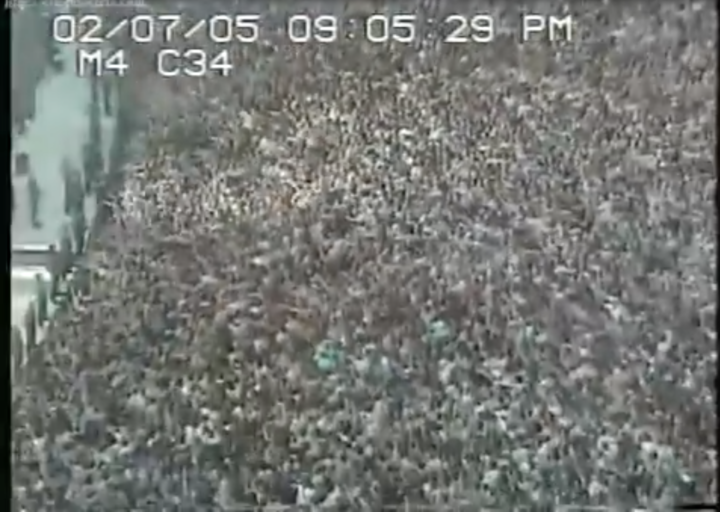
\includegraphics[width=12cm]{img/srowd.png}\\
    Figure 1 - Oasis concert in Manchester, England in 2005
\end{center}
If a mechanical wave propagates in a solid thin rod, the speed of sound is determined by the Newton-Leibniz equation:
\[ c = \sqrt{\frac{E}{\rho}}\]
where: c - speed of sound\\
E - Young modulus\\
$\rho$ - Material density\\\\
The average crowd density can be calculated as:
\[ \rho=\frac{m \cdot d }{h}=\frac{62kg \cdot 3.43 m \textsuperscript{-2}}{1.72 m}=123.64\frac{kg}{m \textsuperscript{3}}\]
where: m - average human mass\\
d - planar crowd density (people per square meter)\\
h - average human height\\\\
Thus, from the Newton-Leibniz equation:
\[ E = c\textsuperscript{2} \cdot \rho = 10.43\frac{m\textsuperscript{2}}{s\textsuperscript{2}} \cdot 123.64\frac{kg}{m \textsuperscript{3}} = 1290 \frac{N}{m\textsuperscript{2}}\]\\
Therefore, it is possible to compute human to human the stiffness coefficient as:
\[K = \frac{E\cdot S}{L}\]
where: S - average square of interaction between two humans\\
L - average distance between two people\\\\
At the same time, an average square of interaction between two humans can be computed as a multiplication between the average human height and the average distance between two humans. Then stiffness coefficient is equal to:
\[K = E \cdot h = 1290 \frac{N}{m\textsuperscript{2}} \cdot 1.72 m = 2219\frac{N}{m}\]
 It is possible to build a mass-spring-dumper chain (figure 2) with obtained elasticity and average human mass, to simulate generalized crowd behavior.
 \begin{center}
    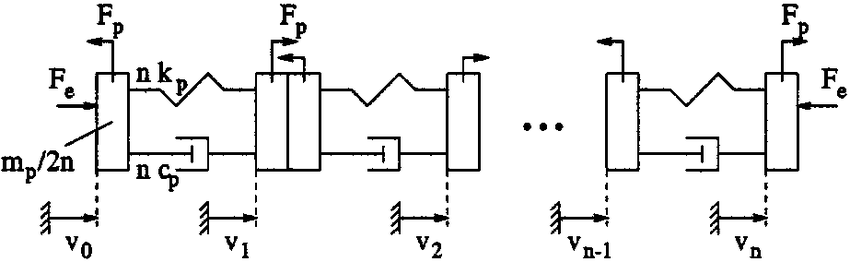
\includegraphics[width=12cm]{img/Model.png}\\
    Figure 2 - Mass-spring-damper chain
\end{center}
\[m \ddot x + b \dot x + Kx = 0\]
where x - vector of humans positions\\
b - damper factor\\\\
It is impossible to find the damper factor in the studied video because the crowded area was smaller than the wave-decreasing length. But it is understandable that it is small enough for our study. On the other side, the damping factor is important for system stability. It is necessary to set damping factor based on heuristic considerations such small that the general behavior was the same or changed insignificantly.\\\\
Let's check the correctness and applicability of assumptions by making a computer model based on obtained parameters and measuring wave velocity.
Let's make a virtual area 10 by 3 meters (figure 3) to do that. It must contend $3.43\cdot10\cdot3=103$ people. It makes up 3.4 meters per second. It is faster by 5\% than the original one. The deviation is due to measurement error.
\begin{center}
    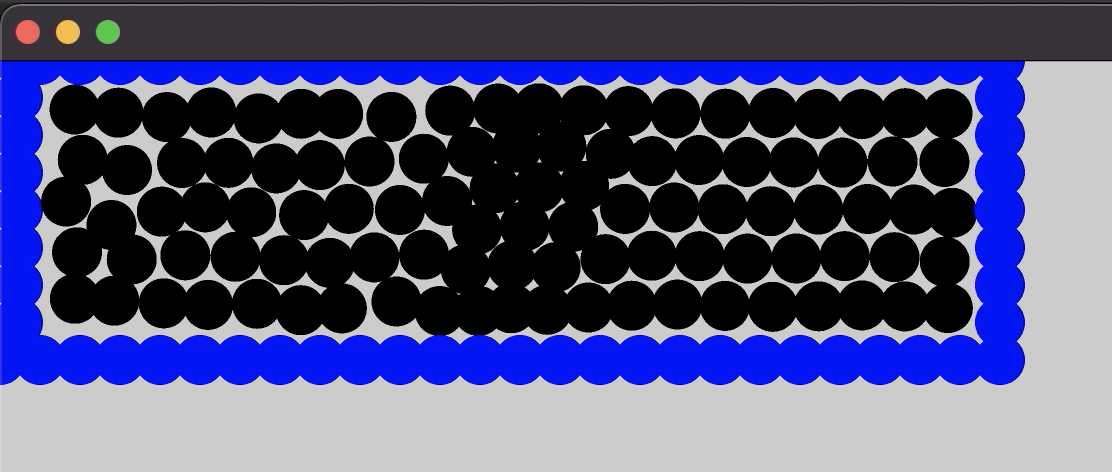
\includegraphics[width=12cm]{img/Wave.png}\\
    Figure 3 - Crowd model (wavefront in the middle)
\end{center}
\chapter*{Crowd control}
Crowd control consists of several steps: node localization, crowd detection, area exploration, and crowd management. \\\\
The considered system consists of low-power, cheap, short-range transmitters (that will be called nodes) and coordinators. It is assumed that everybody in the crowd is equipped with transmitters. The police officers are equipped with smartphones (coordinators) that are able to communicate with transmitters and are able to define their position (via GPS). 
Thus, by communicating one with another, nodes are able to localize their positions with respect to other nodes and coordinators.
\section*{Node localization}
Let's make several assumptions for the section:
\begin{enumerate}
    \item All packages reach their destinations (no transmission loss)
    \item Every device can get a list of available devices in a range
    \item Coordinators know their positions exactly
    \item All nodes are able to communicate very fast. Therefore, every node know everything about all nodes in the system immediately.
\end{enumerate}
The node's position can be founded by overlaying transmitter ranges with the other nodes from the different positions (figure 4). The more devices can detect nodes in their ranges, the more accurate position will be.
\begin{center}
    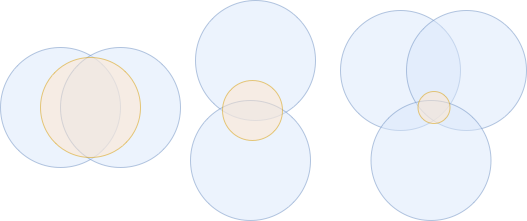
\includegraphics[width=12cm]{img/areas.png}\\
    Figure 4 - Range's overlays (Blue - ranges, Red - estimation)
\end{center}
Every node receives a lot of data from nodes around. All this data is a list of range circles where one node was able to detect the other. Step by step, every node is narrowing the localization circle (figure 5). It is a simple geometrical task - Find the height (h) of the triangle, if all sides are known: radiuses $r1, r2$ and distance between centers $dist$.
\[ p = \frac{(r1+r2+dist)}{2}\]
\[ h = \frac{2\cdot\sqrt{p\cdot(p-dist)\cdot(p-r1)\cdot(p-r2)}}{dist})\]
where: p - half of the triangle's perimeter 
\begin{center}
    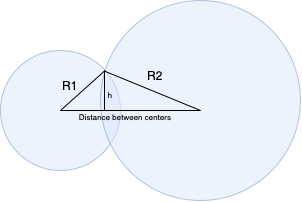
\includegraphics[width=12cm]{img/Geometry.png}\\
    Figure 5 - Circle's narrowing
\end{center}
It is important to notice, that nodes are not able to know their position when they generate a range circle for the other node. Then the circle of the possible node's position sum with a range circle (figure 6).
\begin{center}
    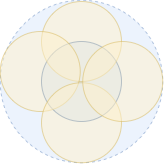
\includegraphics[width=6cm]{img/sum.png}\\
    Figure 6 - Circle sum (blue - position circle, yellow - possible range circles, dashed - resultant)
\end{center}

A lot of plots...A lot of plots...A lot of plots...A lot of plots...A lot of plots...A lot of plots...A lot of plots...A lot of plots...A lot of plots...A lot of plots...A lot of plots...A lot of plots...A lot of plots...A lot of plots...A lot of plots...A lot of plots...A lot of plots...A lot of plots...\\\\
And conclusions...
\section*{Crowd detection}
To detect crowds several technics might be used:
\begin{enumerate}
    \item Based on the number of nodes in transmit range
    \item Based on the short distance with neighbor's nodes
    \item Based on intersections of clouds of locations probability
\end{enumerate}
To be continued...  To be continued...  To be continued...  To be continued...  To be continued...  To be continued...  To be continued...  To be continued...  To be continued...  To be continued...  To be continued...  To be continued...  To be continued...  To be continued...  To be continued...  
\section*{Area exploration}
The crowd uses all available space. Moreover, usually, local authorities prepare additional space for people. All those aspects are hard to take into account before the event. Thus, the system must be adaptive and flexible in terms of available space. \\\\
By storing its positions and sharing them with the other nodes, it is possible to compute the map of available the area. The map will be adaptive in terms of changing: police barriers, cars, gates, etc.












\chapter*{Bibliography}


\end{document}
